%======================================================================
\chapter{Introduction}
%======================================================================

%----------------------------------------------------------------------
\section{Motivation}

% insert robot.png
\begin{figure}[htbp]
    \centering
    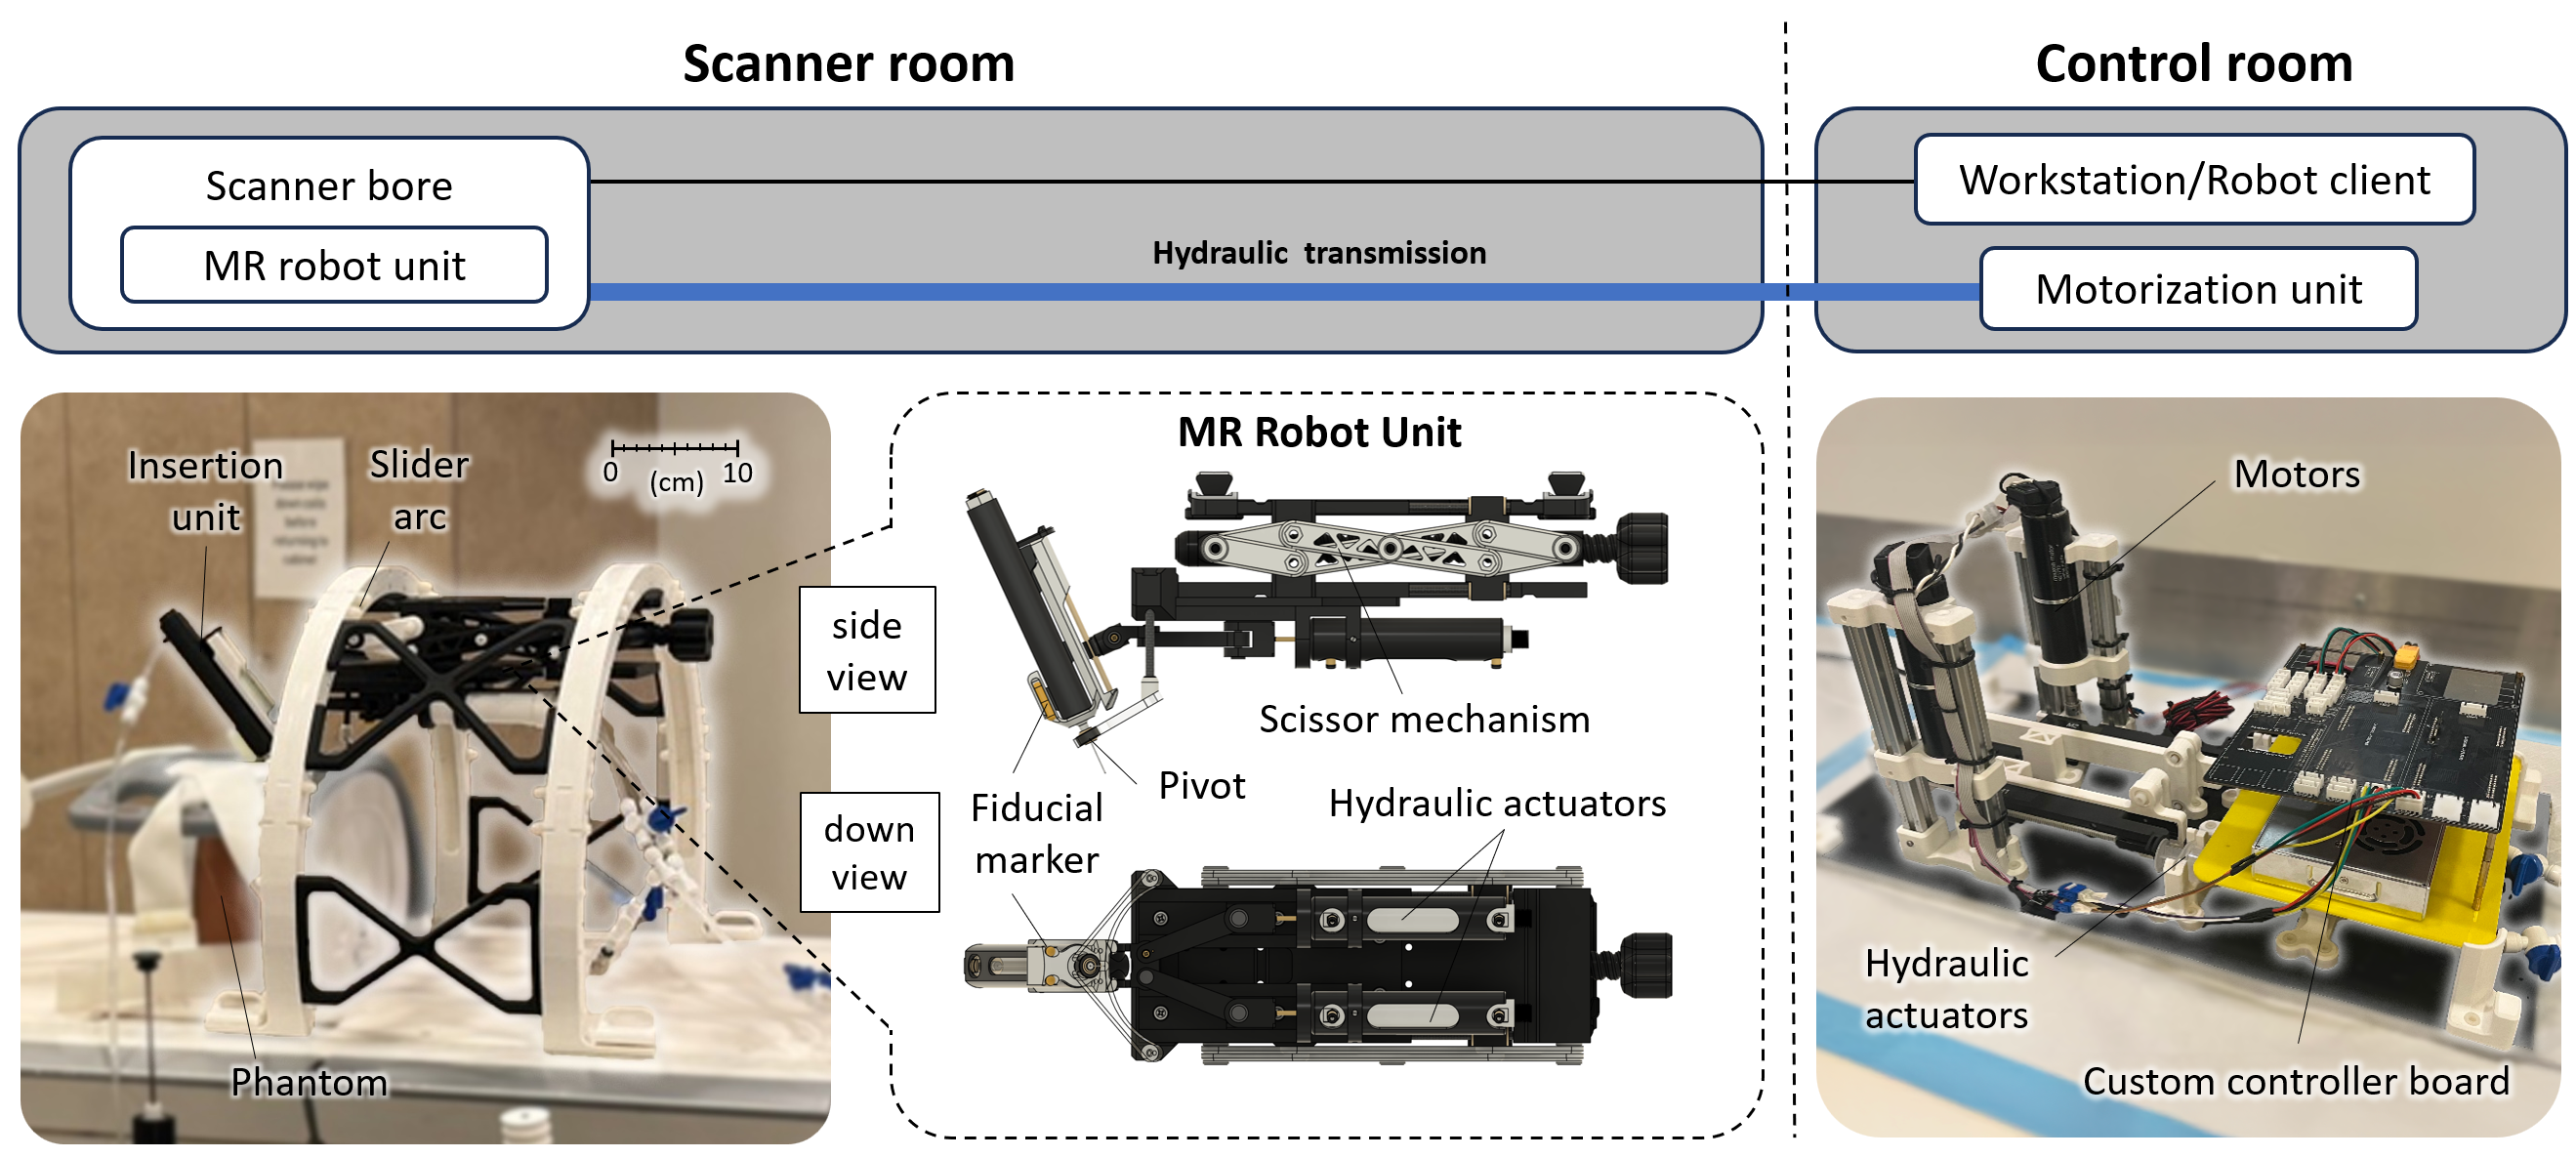
\includegraphics[width=1.0\textwidth]{figures/robot.png}
    \caption{MRI-guided microwave thermal ablation system.}
    \label{fig:robot}
\end{figure}

Liver cancer is among the leading causes of cancer-related mortality
worldwide.
Minimally invasive thermal ablation—delivering focused energy to destroy
tumor tissue without open surgery—is a standard treatment for unresectable
hepatocellular carcinoma~\cite{diederich2005thermal}.
Microwave ablation (MWA) deposits energy through dielectric heating and
produces predictable, roughly ellipsoidal ablation zones on the order of
\SIrange{2}{4}{\cm} in diameter.

\gls{mri} guidance is attractive because it provides superior soft-tissue
contrast, three-dimensional volumetric imaging, and real-time temperature
mapping via \emph{MR thermometry} (proton resonance frequency shift)~\cite{huang2023mri}.
This combination—MWA plus MRI thermometry—creates a closed-loop opportunity:
the power schedule can be updated in real time based on measured temperature,
enabling precise ablation of the tumor while sparing healthy tissue.

%----------------------------------------------------------------------
\section{Problem Statement}

Given the temperature field measured by MRI thermometry, we seek a power
schedule $P(t) \in [0, P_{\max}]$ that:
\begin{enumerate}
    \item achieves complete thermal ablation of the tumor
          ($\Omega_d(\mathbf{r}, t_f) \geq 1$ for all $\mathbf{r} \in \Omega_T$);
    \item keeps healthy tissue below a safety temperature
          ($T(\mathbf{r},t) \leq T_{\text{safe}}$ for all $\mathbf{r} \in \Omega_H$);
    \item minimizes treatment duration and total energy deposition.
\end{enumerate}
This is a \gls{pde}-constrained \gls{ocp} with free final time,
state and control constraints, and a Bolza cost structure.

%----------------------------------------------------------------------
\section{Related Work}

Bioheat equation-based treatment planning dates to the work of
Pennes~\cite{pennes1948analysis}, while the Arrhenius thermal-damage
model used to quantify irreversible necrosis follows
Henriques and Moritz~\cite{moritz1947studies}.
Model-based optimal control approaches have since been applied to
radiofrequency and microwave ablation~\cite{diederich2005thermal} and to
laser interstitial therapy~\cite{feng2011model}, and adjoint-based
gradient methods for \gls{pde}-constrained control are treated
in~\cite{troltzsch2010optimal}.
The optimal-control formulation in this report follows the classical
treatment of the Pontryagin maximum principle and direct
transcription~\cite{pontryagin2018mathematical, kirk1970optimal,
liberzon2012calculus, biegler2010nonlinear}.
The present work integrates these threads into a unified simulation
framework with three solver modes (open-loop, indirect PMP, direct NLP)
and benchmarks them under matched conditions across dimensionality and
probe geometry.

%----------------------------------------------------------------------
\section{Contributions}

The main contributions of this project are:
\begin{enumerate}
    \item A 2-D and 3-D finite-difference simulator of the Pennes bioheat
          PDE and Arrhenius damage ODE, with a free-final-time formulation,
          parameterized by a single configuration object with no magic
          numbers.
    \item An adjoint (costate) solver derived from the \gls{pmp} and
          verified against finite-difference gradient checks.
    \item Three interchangeable solver backends—open-loop, indirect
          gradient projection, and direct single-shooting NLP—sharing a
          common result interface.
    \item Configurable boundary conditions (Dirichlet / Neumann / Robin)
          selectable at the command line.
    \item A quantitative $4 \times 2 \times 3$ sweep (solver $\times$
          dimension $\times$ probe geometry) on a standard
          5~cm $\times$ 5~cm phantom with an 8~mm tumor, identifying when
          each solver and SAR geometry succeeds or fails.
\end{enumerate}

%----------------------------------------------------------------------
\section{Report Organization}

Chapter~\ref{ch:problem} states the mathematical problem.
Chapter~\ref{ch:methods} describes the numerical methods and software
architecture.
Chapter~\ref{ch:results} presents simulation results.
Chapter~\ref{ch:conclusion} concludes and outlines future work.
